\subsection{Graphical Representations}

We can represent the qualitative structure of an iSCM by means of graphs.
The directed edges in such a graph will express the following ``parent''-relation that captures \emph{functional dependencies} in the structural equations / causal mechanisms of the iSCM.
\begin{Def}\label{def:scm_parent}
  Let $M = \lt \Sin, \Send, \Srnd, \CX, P, f \rt$ be an iSCM.
  For $i \in \Sin \cup \Send \cup \Srnd$ and $j \in \Send$, we say that
  \emph{$i$ is a parent of $j$ according to $M$} if there does not exist a measurable function 
  $\tilde f_j : \CX_{(\Sin\cup\Send\cup\Srnd) \setminus \{i\}} \to \CX_j$
  such that
  $$x_j = f_j(x) \iff x_j = \tilde f_j(x_{\setminus i}) \qquad M\as,$$
  where $x_{\setminus i}$ is shorthand for $x_{(\Sin\cup\Send\cup\Srnd)\setminus\{i\}}$.
\end{Def}
In words, $i$ is a parent of $j$ if the solutions of the structural equation for $j$ essentially depend on the value of variabe $i$.
By definition, exogenous (input and random) variables have no parents.
%Note that the parent-relationship is preserved under equivalence.

Using directed edges to encode the parent-relationship, we define two graphical representations.
The more fine-grained representation represents all the variables as nodes.
We will also frequently use a coarser representation that represents only 
the endogenous variables and the exogenous input variables as nodes (but not the exogenous random variables).
\begin{Def}\label{def:scm_graph}
  Let $M = \lt \Sin, \Send, \Srnd, \CX, P, f \rt$ be an iSCM.
  The CDG $\lt \Sin, \Send \cup \Srnd, E \rt$ with
  input nodes $\Sin$, output nodes $\Send\cup\Srnd$, and
  directed edges 
  $$E = \{i \tuh j : i \in \Sin\cup\Srnd\cup\Send, j\in\Send: \text{$i$ is parent of $j$ according to $M$}\}$$
  is called the \emph{graph of the iSCM} and will be denoted as $G^+(M)$.

  The marginalized graph $(G^+(M))^{\setminus W}$ in which all exogenous random nodes have been marginalized out (via Definition~\ref{def:G_marginalization}), will be called the \emph{causal graph of the iSCM} and denoted as $G(M)$.\footnote{The reason we use the adjective ``causal'' is to emphasize that every node in the causal graph has a causal interpretation, as the corresponding variable can be targeted by a hard intervention.}
\end{Def}
%While the graph explicitly represents all exogenous random variables, coarser
%representations obtained via (graphical) marginalization are also useful.
\begin{Rem}\label{rem:scm_graph}
%  An often used convention is to consider \emph{all} exogenous random variables to be latent. 
%  In that case, a useful graph
%  to consider is the marginalization $G^{\setminus \Srnd}(M)$ of the graph $G(M)$. 
  The causal graph $G(M) = \lt \Sin, \Send, E, L \rt$ has input nodes $\Sin$, output nodes $\Send$, directed edges
  $$E = \{i \tuh j : i \in \Sin\cup\Send, j\in\Send: \text{$i$ is parent of $j$ according to $M$}\}$$
  and bidirected edges
  $$L = \{j \huh k : j \in \Send, k \in \Send, j \ne k: \text{$j$ and $k$ have a common parent in $W$ according to $M$}\}.$$
  In other words, $G(M)$ is obtained from $G^+(M)$ by replacing the nodes representing the exogenous random
  variables and their outgoing directed edges with bidirected edges, i.e.,
  any pattern $\hut w \tuh$ with $w \in \Srnd$ is replaced by $\huh$.
\end{Rem}

%Since the parent-relationship is preserved under equivalence, equivalent iSCMs have the same graphs.
Note that observably equivalent iSCMs may have different graphs, and even interventionally equivalent iSCMs may have different graphs. % Note that in the following example, even node-splitting interventions will not allow us to distinguish the two models
\begin{Eg}\label{eg:interventionally_equivalent_but_different_graphs}
Consider the SCM $M$ with endogenous variables $X_1,X_2,X_3$ with co-domains $\{-1,1\}$, $\{-1,1\}$, $\{-2,0,2\}$, respectively, and structural equations
$$
  \begin{aligned} 
    X_1 &= X_A \\
    X_2 &= X_1 X_B \\
    X_3 &= X_2 + X_B,
  \end{aligned} 
$$
with independent exogenous random variables $X_A,X_B \sim \mathrm{Uni}(\{-1,1\})$.
Its graph $G^+(M)$ and its causal graph $G(M)$ are depicted in Figure~\ref{fig:interventionally_equivalent_but_different_graphs} (left top and bottom, respectively).

\begin{figure}
  \begin{center}
    \begin{tikzpicture}
      \begin{scope}[xshift=0]
        \node[ndout] (X1) at (0,0) {$X_1$};
        \node[ndout] (X2) at (2,0) {$X_2$};
        \node[ndout] (X3) at (4,0) {$X_3$};
        \node[ndlat] (E1) at (0,1.5) {$X_A$};
        \node[ndlat] (E2) at (3,1.5) {$X_B$};
        \draw[arout] (E1) -- (X1);
        \draw[arout] (X1) -- (X2);
        \draw[arout] (X2) -- (X3);
        \draw[arout] (E2) -- (X2);
        \draw[arout] (E2) -- (X3);
        \node at (2,-1.5) {$G^+(M)$};
      \end{scope}
      \begin{scope}[yshift=-3cm]
        \node[ndout] (X1) at (0,0) {$X_1$};
        \node[ndout] (X2) at (2,0) {$X_2$};
        \node[ndout] (X3) at (4,0) {$X_3$};
        \draw[arout] (X1) -- (X2);
        \draw[arout] (X2) -- (X3);
        \draw[arlat,bend left] (X2) edge (X3);
        \node at (2,-1.5) {$G(M)$};
      \end{scope}
      \begin{scope}[xshift=8cm]
        \node[ndout] (X1) at (0,0) {$X_1$};
        \node[ndout] (X2) at (2,0) {$X_2$};
        \node[ndout] (X3) at (4,0) {$X_3$};
        \node[ndlat] (E1) at (0,1.5) {$X_A$};
        \node[ndlat] (E2) at (3,1.5) {$X_C$};
        \draw[arout] (E1) -- (X1);
%        \draw[arout] (X1) -- (X2);
        \draw[arout] (E2) -- (X2);
        \draw[arout,bend right] (X1) edge (X3);
        \draw[arout] (X2) -- (X3);
        \draw[arout] (E2) -- (X3);
        \node at (2,-1.5) {$G^+(\tilde{M})$};
      \end{scope}
      \begin{scope}[xshift=8cm,yshift=-3cm]
        \node[ndout] (X1) at (0,0) {$X_1$};
        \node[ndout] (X2) at (2,0) {$X_2$};
        \node[ndout] (X3) at (4,0) {$X_3$};
        \draw[arout,bend right] (X1) edge (X3);
        \draw[arout] (X2) -- (X3);
        \draw[arlat,bend left] (X2) edge (X3);
        \node at (2,-1.5) {$G(\tilde{M})$};
      \end{scope}
    \end{tikzpicture}
  \end{center}
  \caption{The graphs of the interventionally equivalent SCMs $M$ (left) and $\tilde{M}$ (right) corresponding to Example~\ref{eg:interventionally_equivalent_but_different_graphs}. The corresponding causal graphs (that do not represent exogenous random variables as nodes) are shown in the bottom row.\label{fig:interventionally_equivalent_but_different_graphs}}
\end{figure}
Consider also the SCM $\tilde{M}$ with endogenous variables $X_1,X_2,X_3$ with co-domains $\{-1,1\}$, $\{-1,1\}$, $\{-2,0,2\}$, respectively, and structural equations
$$
  \begin{aligned} 
    X_1 &= X_A \\
    X_2 &= X_C \\
    X_3 &= X_2 + X_1 X_C,
  \end{aligned} 
$$
with independent exogenous random variables $X_A,X_C \sim \mathrm{Uni}(\{-1,1\})$.
Its graph $G^+(\tilde{M})$ and causal graph $G(\tilde{M})$ are depicted in Figure~\ref{fig:interventionally_equivalent_but_different_graphs} (right top and bottom, respectively).
$\tilde{M}$ was obtained from $M$ by making a change of variables $x_C = x_1 x_B$.
One can check that $\tilde{M}$ is interventionally equivalent to $M$ (with respect to
$\{1,2,3\}$), even though its the graph $G^+(M)$ differs from the graph $G^+(\tilde{M})$,
and its causal graph $G(M)$ differs from the causal graph $G(\tilde{M})$.\footnote{Even node-splitting interventions would not allow to distinguish the two SCMs.
\Joris{Interestingly, ``rich node-splitting interventions'' inspired by Sander, where we are allowed to split a node into separate copies that enter each of its descendants, would allow us to distinguish them!
This yields the conjecture that the graph \emph{is} identifiable under these ``rich node-splitting interventions''.
It also suggests that the term ``interventionally equivalent'' is not adequate as it lacks precision.
But whether this is an empirically realistic type of intervention is not completely clear at the moment.}
\Joris{Also, perhaps the two SCMs could be distinguished with node-splitting interventions where one sets
the value of the later copy as a function of the ancestors of the earlier copy?}
%and the marginal graph $G(M)^{\sm \{A,B\}}$ differs from the marginal graph $G(\tilde{M})^{\sm \{A,C\}}$.
\Joris{It is relatively easy to see that node-splitting interventions won't help to distinguish the two.
First of all, we don't need to split $X_1$ because the two models are identical on $X_1$ and its ancestors.
We also don't need to split $X_3$ because $X_3$ has no children in both models.
If we split $X_2$ then we can easily see that for $M$ we have $X_3 = X_2^1 + X_2^0 X_1$ and $(X_1,X_2)$ uniformly distributed, 
whereas for $\tilde{M}$ we also have $X_3 = X_2^1 + X_2^0 X_1$ and $(X_1,X_2)$ uniformly distributed.}
}
\end{Eg}

\begin{Rem}\label{rem:iscm_structurally_minimal}
  Let $M = \lt \Sin, \Send, \Srnd, \CX, P, f \rt$ be an iSCM and let $G^+ := G^+(M)$ be its graph.
  Then there exists an equivalent iSCM $\tilde{M} \equiv M$ with causal mechanism $\tilde{f} : \CX \to \CX_V$ such that for each $v \in V$:
  $\tilde f_v$ is constant in $x_{(J \cup W \cup V) \sm \Pa^{G^+}(v)}$.
  Hence, the causal mechanisms of $\tilde{M}$ can be seen as a tuple of functions $(\tilde f_v : \CX_{\Pa^{G+}(v)} \to \CX_v)_{v \in V}$.
\end{Rem}
In the literature, things are often done in the opposite way: given a graph, one considers an SCM such that its causal mechanisms respect the graph structure.

We already provided definitions for hard interventions on graphs (Definition~\ref{def:G_hard_intervention})
and for marginalizations (latent projections) of graphs (Definition~\ref{def:G_marginalization}). 
The mapping that maps an iSCM to its graph is compatible with the elementary operations on iSCMs and on graphs.
\begin{Prp}\label{prp:compatibility_graph}
  Let $M = \lt \Sin, \Send, \Srnd, \CX, P, f \rt$ be an iSCM. Then
  \begin{itemize}
    \item Hard interventions: for $T \subseteq J \cup V$, 
      $$G^+(M_{\doit(T)}) = (G^+(M))_{\doit(T)} \qquad \text{and} \qquad G(M_{\doit(T)}) = (G(M))_{\doit(T)}.$$
    \item Marginalizations: If $M$ is simple, then for $L \subseteq V$, 
      $$G^+(M_{\setminus L}) \subseteq (G^+(M))^{\setminus L} \qquad \text{and} \qquad G(M_{\setminus L}) \subseteq (G(M))^{\setminus L}.$$
  \end{itemize}
\end{Prp}
\begin{proof}
  The first statement follows by writing out the definitions. 
  
  The second statement is somewhat more involved. We will
  first prove it in case $L = \{\ell\}$ consists of a single node. 
  Let $G^+ := G^+(M)$.
  By using the definition of the parent relation (repeatedly), we can find a function $\tilde{f}_\ell : \CX_{\Pa^{G^+}(\ell)} \to \CX_\ell$ such that:
  $$x_\ell = f_\ell(x) \iff x_\ell = \tilde{f}_\ell(x_{\Pa^{G^+}(\ell)})\quad M\as.$$
  Since $\ell \notin \Pa^{G^+}(\ell)$ because $M$ is simple (see Proposition~\ref{prp:self-cycles}), %(more generally: because $M_{\doit(V\setminus\{\ell\})}$ is uniquely solvable),
  the essentially unique solution function
  $\tilde{g}_\ell : \CX_{J \cup V \setminus \{\ell\} \cup W} \to \CX_\ell$ of $M_{\doit(V\setminus \{\ell\})}$
  satisfies $\tilde{g}_\ell(x_{\setminus \ell}) = \tilde{f}_\ell(x_{\Pa^{G^+}(\ell)})\ M\as$, i.e., it only depends on the parents of $\ell$.
  When constructing the marginalized causal mechanism for $M_{\setminus \{\ell\}}$, we substitute 
  $\tilde{g}_\ell(x_{\setminus \ell})$ into the $\ell$'th input of the causal mechanism $f_j$ of $M$, for $j \in V\setminus \{\ell\}$.
  Since $\tilde{g}_\ell$ only depends on $\Pa^{G^+}(\ell)$,
  we get that $\Pa^{\tilde G^+}(j) \subseteq \Pa^{G^+}(j) \setminus \{\ell\} \cup \Pa^{G^+}(\ell)$, where $\tilde{G}^+ = G^+(M_{\setminus \ell})$.
  But we also have $\Pa^{(G^+)^{\setminus \{\ell\}}}(j) = \Pa^{G^+}(j) \setminus \{\ell\} \cup \Pa^{G^+}(\ell)$ by definition of the graphical marginalization. 
  Hence $\Pa^{\tilde G^+}(j) \subseteq \Pa^{(G^+)^{\setminus \{\ell\}}}$ for all $j \in V\setminus \{\ell\}$, and we have shown that $G^+(M_{\setminus \{\ell\}}) \subseteq (G^+(M))^{\setminus \{\ell\}}$.
  For the general case, we can make use of induction and the facts that both for
  graphs and simple iSCMs, we can obtain a marginalization over a subset by repeatedly marginalizing out a single remaining node in the subset, in arbitrary order.
  Finally, note that $G(M_{\sm L}) = (G^+(M_{\sm L}))^{\sm W} \subseteq ((G^+(M))^{\sm L})^{\sm W} = G(M)^{\sm L}$.
\end{proof}
\begin{Rem}
  When working with $G^+(M)$, which contains no bidirected edges by definition, and marginalizing out a subset of nodes $L \ins V$, there is actually no need to add any bidirected edges.
  Once the first node in $W$ has been marginalized out, though, adding bidirected edges when marginalizing out further nodes becomes necessary.
  Hence, our definition of graphical marginalization is somewhat conservative, as it may add more bidirected edges than necessary in general.
  An alternative approach could be to distinguish ``deterministic nodes'' (which represent variables that are deterministic functions of their parents) from ``stochastic nodes'' in a graph.
  This allows one to track more accurately whenever there is a need to add bidirected edges when marginalizing out a subset of nodes.
  The reason that we chose the more conservative approach instead is that in practice, we often model a causal system by means of the causal graph $G(M)$; as the causal graph does not specify which of its nodes are deterministic, we end up making the worst-case assumption that all of its nodes are stochastic.
\end{Rem}

\subsection{Self-Cycles}
%\begin{Exc}
%  Do graphs of counterfactually equivalent SCMs have the same directed edges between endogenous variables?
%  Give a proof or a counterexample.
%\end{Exc}
\begin{figure}
  \begin{center}\begin{tikzpicture}
    \begin{scope}
      \node at (-1,0) {(a)};
      \node[ndlat] (W) at (0,0) {$W$};
      \node[ndout] (X) at (1.5,0) {$X$};
      \draw[arout] (W) -- (X);
    \end{scope}
    \begin{scope}[xshift=6cm]
      \node at (-1,0) {(b)};
      \node[ndlat] (W) at (0,0) {$W$};
      \node[ndout] (X) at (1.5,0) {$X$};
      \draw[arout] (W) -- (X);
  %    \draw[arout,in=30,out=-30,looseness=5] (X) edge (X);
      \draw[arout,looseness=5] (X) edge (X);
    \end{scope}
  \end{tikzpicture}\end{center}
  \caption{Graphs without and with a self-cycle in Example~\ref{eg:self_cycle}.\label{fig:eg:self_cycle}}
\end{figure}
Our goal was to allow for possible cycles in an iSCM. This means that we may also encounter \emph{self-cycles}.
\begin{Eg}\label{eg:self_cycle}
  Consider an SCM with an endogenous variable $X \in \RN$ and an exogenous random variable $W \in \RN$.

  If it has structural equation
  $$X = X -X^3 + W,$$
  %is equivalent to the SCM obtained by replacing the structural equation with
  %$$X = \sqrt[3]{W}.$$
  %Note that $X$ no longer appears on the r.h.s..
  %with endogenous variable $X \in \RN$ and exogenous random variable $W \in \RN$ and structural equation
  then its graph is the one in Figure~\ref{fig:eg:self_cycle}(a).
  In particular, it does not have a self-cycle at $X$, since $X$ is not a parent of itself. 
  Indeed, the structural equation is equivalent to 
  $$X = \sqrt[3]{W},$$
  where $X$ does not appear on the r.h.s..
  
  On the other hand, if it has structural equation
  $$X = X -X^2 + W^2,$$
%  $$X = W X + c,$$
%  is not equivalent to the SCM obtained by replacing the structural equation with
%  $$X = \begin{cases}
%          \xi & W = 1 \\
%          \frac{c}{1 - W} & W \ne 1
%        \end{cases}$$
%  no matter how we choose $\xi$, even when $P(W=1) = 0$. 
  then its graph is the one in Figure~\ref{fig:eg:self_cycle}(b), which in particular contains a self-cycle at $X$.
\end{Eg}
Self-cycles complicate matters because they indicate solvability issues.

To understand why self-cycles are in some sense inevitable, consider an SCM with structural equations
\begin{align*}
  X_1 &= X_2 \\
  X_2 &= X_3 \\
  X_3 &= X_1 
\end{align*}
Marginalizing out $X_2$ and $X_3$ gives an SCM with structural equation
$$X_1 = X_1,$$
which turns the cycle $X_1\tuh X_3 \tuh X_2\tuh X_1$ into a self-cycle $X_1\tuh X_1$.
Self-cycles are of no concern, though, when restricting to the class of simple iSCMs.
\begin{Prp}\label{prp:self-cycles}
  Let $M$ be an iSCM.
  For $j \in V$, there is a self-cycle $j \tuh j$ in $G^+(M)$ if and only if
  $M$ is \emph{not} essentially uniquely solvable w.r.t.\ $j$. 
  In particular, graphs of simple iSCMs have no self-cycles.
\end{Prp}
\begin{proof}
  $j$ is not a parent of itself according to $M$ iff there is a function $\tilde f_j : \CX_{(\Sin\cup\Send\cup\Srnd) \setminus \{j\}} \to \CX_j$ such that $x_j = f_j(x) \iff x_j = \tilde f_j(x_{\setminus j})\ M\as,$ which holds iff $M$ is essentially uniquely solvable w.r.t.\ $j$.
\end{proof}

\begin{figure}[t]\centering
  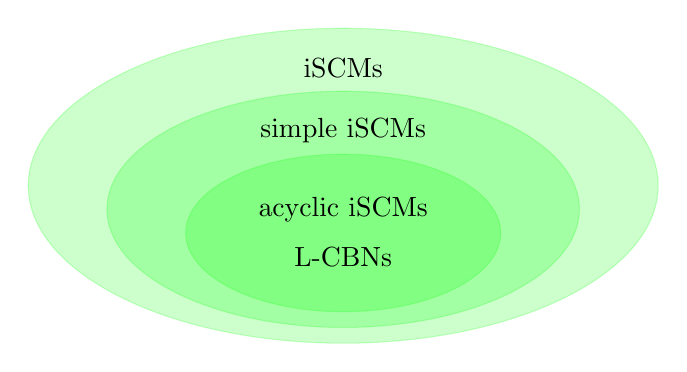
\begin{tikzpicture}
      \begin{scope}
%        \draw[draw=green,fill=green,opacity=0.2] (0,0) ellipse (1.5cm and 0.5cm);
        \draw[draw=green,fill=green,opacity=0.2] (0,0.3) ellipse (2cm and 1cm);
        \draw[draw=green,fill=green,opacity=0.2] (0,0.6) ellipse (3cm and 1.5cm);
        \draw[draw=green,fill=green,opacity=0.2] (0,0.9) ellipse (4cm and 2cm);
        \node at (0,0) {L-CBNs};
        \node at (0,0.6) {acyclic iSCMs};
        \node at (0,1.6) {simple iSCMs};
        \node at (0,2.4) {iSCMs};
      \end{scope}
  \end{tikzpicture}
  \caption{Venn diagram for different causal modeling classes.\label{fig:venn_diagram_scms}}
\end{figure}

\subsection{Acyclic iSCMs}\label{sec:acyclic_scms}
A subclass of iSCMs that is often considered are acyclic iSCMs.
\begin{Def}\label{def:scm_acyclic}
  An iSCM $M$ is called \emph{acyclic} if its graph $G^+(M)$ is acyclic.
\end{Def}
Note that this holds if and only if its causal graph $G(M)$ is acyclic.
If one models static systems, then using acyclic iSCMs
rules out the presence of causal cycles (e.g., feedback loops) in the system.
Acyclic iSCMs are a subclass of the more general class of simple iSCMs.
\begin{Prp}\label{prp:acyclic_scms_are_simple}
  Acyclic iSCMs are simple.
\end{Prp}
\begin{proof}
  We first show that acyclic iSCMs are essentially uniquely solvable. Let $M$ be an acyclic iSCM. Its
  graph $G^+ := G^+(M)$ is acyclic, and hence has a topological order $<$. Consider $f_v$, the
  causal mechanism for $v \in V$. The parents $\Pa^{G^+}(v)$ precede $v$ in the topological order.
  Without loss of generality, we may assume that each mechanism $f_v$ only depends on its parents
  (see Remark~\ref{rem:iscm_structurally_minimal}), and thus consider $f_v : \CX \to \CX_v$ as a function
  $f_v : \CX_{\Pred_<^{G^+}(v)} \to \CX_v$ instead. We can then inductively define the components
  $$g_v : \CXJ \times \CXW \to \CX_v : 
    (\xJ,\xW) \mapsto f_v(g_{\Pred_<^{G^+}(v)}(\xJ,\xW))$$
  that together form a solution function $g : \CX_{J\cup W} \to \XV$.
  This construction also exhibits the essential uniqueness of $g : \CX_{J\cup W} \to \XV$.

  Next consider $M_{\doit(T)}$, the intervened iSCM for a hard intervention on $M$ with target $T \subseteq V$. 
  It has graph $G^+(M_{\doit(T)}) = (G^+)_{\doit(T)}$, whose edges form a subset of the edges of $G^+$ (but
  where some output nodes have become input nodes), and hence is also acyclic. 
  Therefore, also $M_{\doit(T)}$ is essentially uniquely solvable. 
  One easily sees that the solution function constructed above is also a partial solution function of $M$ w.r.t.\ $V \sm T$,
  which is essentially unique.
  \Claude{The proof that the solution of $M_{\doit(T)}$ also serves as a partial solution function of~$M$ w.r.t.~$T$ is stated but not fully detailed.}
  \Joris{TODO: Hm, we may need to proceed more carefully here, and above.}
  Since this holds for all targets $T \subseteq V$, we conclude that $M$ is simple.
\end{proof}

%\subsection{Interventional equivalence of acyclic iSCMs and (L-)CBNs}\label{sec:interventional_equivalence_scms_cbns}

Figure~\ref{fig:venn_diagram_scms} shows a Venn diagram to illustrate the relationships between the different
classes of causal models that we introduced.
We will show that in a precise sense, acyclic iSCMs and L-CBNs are equally expressive.
\begin{Def}\label{def:interventional_equivalence_cbn_scm}
  Let $M = \lt \Sin, \Send, \Srnd, \CX, P, f \rt$ be a simple iSCM and let $\tilde{M}$ be an L-CBN with graph
  $\tilde{G}^+ = (\tilde{J},\tilde{V}\dcup\tilde{U},\tilde{E})$, spaces $\tilde{\CX}_{\tilde v}$ for $\tilde{v} \in \tilde{V} \cup \tilde{U} \cup \tilde{J}$,
  and Markov kernels $$P_{\tilde{v}}\lp X_{\tilde{v}} | X_{\Pa^{\tilde{G}^+}}(\tilde{v}) \rp.$$
  We say that \emph{$M$ is interventionally equivalent to $\tilde{M}$ w.r.t.\ $O \subseteq V \cap \tilde{V}$} if
  $\CX_O = \tilde{\CX}_O$, $\CX_{J \cap \tilde{J}} = \tilde{\CX}_{J \cap \tilde{J}}$, and
  for any hard intervention $\doit(T)$ with $T \subseteq O$, the intervened Markov kernel $P_M(X_{O\sm T}|\doit(X_{J\cup T}))$ of $M$ equals the intervened Markov kernel $P(X_{O\sm T}|\doit(X_{\tilde{J}\cup T}))$ of $\tilde{M}$.
  %Special case $J = \tilde{J}$, $O = V \cup W$, $\tilde{V} = V \cup W$, $\tilde{U} = \emptyset$:
\end{Def}
\begin{Prp}\label{prp:interventional_equivalence_cbn_scm}
  \begin{enumerate}[label=\roman*)]
    \item Given an acyclic iSCM $M = \lt \Sin, \Send, \Srnd, \CX, P, f \rt$ and a subset $O \subseteq V$, we can construct an L-CBN $\tilde{M}$ with observed output variables $\tilde{V} = O$, latent output variables $\tilde{U} = (V \cup W) \sm O$, input variables $J$, graph $G^+(M)$, and spaces $\CX_v$ for $v \in V\cup W \cup J$ that is interventionally equivalent to $M$ w.r.t.\ $O$.
    \label{prp:interventional_equivalence_cbn_scm:scm2cbn}
    \item Given an L-CBN 
      $\tilde{M} = \lp G^+=(J,(O,U),E^+), \; \lp P_v(X_v| X_{\Pa^{G^+}(v)}) \rp_{v\in O \cup U} \rp$
      with observed variables $O$, we can construct 
%      \begin{enumerate}
%        \item an acyclic iSCM $M$ with input variables $J$, endogenous variables $O \dcup U$ and causal graph $G(M) \subseteq G^+$ that is interventionally equivalent to $\tilde{M}$ w.r.t.\ $O$.
%        \item 
      an acyclic iSCM $M$ with input variables $J$, endogenous variables $O$ and causal graph $G(M) \subseteq (G^+)^{\sm U}$ that is interventionally equivalent to $\tilde{M}$ w.r.t.\ $O$.
%      \end{enumerate}
    \label{prp:interventional_equivalence_cbn_scm:cbn2scm}
  \end{enumerate}
\end{Prp}
\begin{proof}
  \begin{enumerate}[label=\roman*)]
    \item
      Let $M = \lt \Sin, \Send, \Srnd, \CX, P, f \rt$ be an acyclic iSCM with graph $G^+(M) = (J, V \cup W, E)$.
      Define $\tilde{M}$ as the L-CBN with observed output variables $\tilde{V} = O$, latent output variables $\tilde{U} = (V \cup W) \sm O$, input variables $J$, graph $G^+:=G^+(M)$, spaces $\CX_v$ for $v \in V\cup W \cup J$, and the following Markov kernels.
      For $v \in V$, we write its structural equation as:
      $$x_v = f_v(x_{\Pa^{G^+}(v)})$$
      with $f_v : \CX_{\Pa^{G^+}(v)} \to \CX_v$,
      where $v \notin \Pa^{G^+}(v)$ because the graph is acyclic. We then define the corresponding (deterministic) Markov kernel
      \[ P_v\lp X_v|X_{\Pa^{G^+}(v)}\rp := \delta_{f_v}(X_v|X_{\Pa^{G^+}(v)}),\]
      encoding the causal mechanisms of $M$.
      The Markov kernels for $w \in W$ are defined as:
      \[ P_w\lp X_w|X_{\Pa^{G^+}(w)}\rp := P_w(X_w),\]
      encoding the exogenous distributions of $M$, where we note that $\Pa^{G^+}(w) = \emptyset$.
      One can check that this L-CBN $\tilde{M}$ does the job.
    \item
      Let 
      \[ \tilde{M} = \lp G^+=(J,(O,U),E^+), \; \lp P_v(X_v| X_{\Pa^{G^+}(v)}) \rp_{v\in O \cup U} \rp \]
      be an L-CBN.
      For every $v \in O \dcup U$, we can write the Markov kernel $P_v$ as the composition of a deterministic one and 
      a uniform distribution $P_{\bar v}(X_{\bar v})$ on $\Xcal_{\bar v}:=[0,1]$ by Remark \ref{rem:R-to-std-ms}:
        \[ P_v(X_v|X_{\Pa^{G^+}(v)}) = \delta(f_v|X_{\bar v}, X_{\Pa^{G^+}(v)}) \circ P_{\bar v}(X_{\bar v}) \]
      for some measurable function $f_v : \CX_{\bar v} \times \CX_{\Pa^{G^+}(v)} \to \CX_v$.
      Here, we introduced new variables $\bar v$ for each $v \in O \dcup U$.

      Define now the iSCM $\bar{M} = \lt J, O \dcup U, \bar O \dcup \bar U, \CX_J \times \CX_{O \dcup U} \times \CX_{\bar O \dcup \bar U}, P, f \rt$ by taking
      $$P(X_{\bar O \dcup \bar U}) = \bigotimes_{\bar v \in \bar O \dcup \bar U} P_{\bar v}(X_{\bar v})$$
      and
      $$f = (f_v)_{v \in O \dcup U}.$$
      That is, the uniformly distributed random variables $X_{\bar v}$ become the exogenous random variables,
      all independent and uniformly distributed on $[0,1]$, and the components of the causal mechanism correspond to the deterministic functions used to represent the Markov kernels.
      The marginalized iSCM $M := \bar{M}_{\sm U}$ does the job, as one can check.
  \end{enumerate}
\end{proof}
Simple iSCMs are more expressive than acyclic iSCMs because they can model (sufficiently
weak) causal cycles. iSCMs in general are even more expressive because they can also
model stronger cycles that not necessarily lead to unique solvability under any hard
intervention, but this generality comes with a substantially increased complexity of
the theory and interpretability. Simple iSCMs form a ``sweet spot'' in the sense that they allow cyclic
relationships yet their theory is not much more complicated than that of acyclic iSCMs:
the main difference consists in replacing $id$-separation with $i\sigma$-separation.

\begin{Exc}
  Show that all simple iSCMs with two endogenous binary variables $X,Y$ must be acyclic.
  Give an example of a cyclic simple iSCM with two endogenous variables $X,Y$ that take on values in $\{0,1,2\}$.
  % define a MIN b = \max(a-b,0)
  % x = y MIN 1
  % y = x MIN 1
  % unique solution: x=y=0
\end{Exc}

Even iSCMs may not be the ultimate way of modeling cyclic causal systems. Indeed, for such
systems, it might be that the conceptual notion of interventions \emph{targeting variables} is misguided in general, 
and perhaps should be replaced by the notion of intervening on \emph{functional constraints} \cite{BlomVanDiepenMooij_JMLR_21}.

\subsection{Examples}\label{sec:scm_examples}

In many systems occurring in the real world, feedback loops between observed variables are present. 
Such systems can often be described by a system of (random) differential equations. 
The equilibrium states of such systems can sometimes be causally modelled by an iSCM \cite{BM18}.

For illustration purposes we provide two examples, the first consisting of interacting masses that are attached to springs
that can be described at equilibrium with a simple iSCM, the second being the famous price-supply-demand model that has been
very popular in econometrics, and which corresponds to a non-simple SCM at equilibrium.

\begin{Eg}[Damped coupled harmonic oscillator]\label{ex:HarmonicOscillator}
Consider a one-dimensional system of $d$ masses $m_i\in\RN$
($i=1,\dots,d$) with positions $Q_i$. The masses are
coupled by springs, with spring constants $k_i>0$ ($i=0,\dots,d$) and equilibrium lengths $\ell_i>0$
($i=0,\dots,d-1$), under influence of friction with friction coefficients $b_i>0$ ($i=1,\dots,d$).
The endpoints are considered fixed at positions
$Q_0 < Q_{d+1}$ (see Figure~\ref{fig:MassSpringSystem} (top)).
\begin{figure}\centering
  \scalebox{0.8}{\begin{tikzpicture}
    \begin{scope}
      \fill[pattern=north east lines,draw=none] (-1,-1) rectangle (0,1);
      \draw (0,-1) -- (0,1);
      \begin{scope}[yshift=5mm]
      \node (Q1) at (2,0) {$m_1$};
      \node (Q2) at (4,0) {$m_2$};
      \node (Q3) at (6,0) {$m_3$};
      \node (Q4) at (8,0) {$m_4$};
      \node (Q5) at (10,0) {$m_5$};
      \end{scope}
      \begin{scope}[yshift=-5mm]
        \node (l0) at (1,0) {$k_0$};
        \node (l1) at (3,0) {$k_1$};
        \node (l2) at (5,0) {$k_2$};
        \node (l3) at (7,0) {$k_3$};
        \node (l4) at (9,0) {$k_4$};
        \node (l5) at (11,0) {$k_5$};
      \end{scope}
      \fill[black] (2,0) circle (.2);
      \fill[black] (4,0) circle (.2);
      \fill[black] (6,0) circle (.2);
      \fill[black] (8,0) circle (.2);
      \fill[black] (10,0) circle (.2);
      \draw (12,-1) -- (12,1);
      \fill[pattern=north east lines,draw=none] (12,-1) rectangle (13,1);
      \draw[thick,decorate,decoration={coil,aspect=0.7,amplitude=4,segment length=3mm}] (0,0) -- (2,0);
      \draw[thick,decorate,decoration={coil,aspect=0.7,amplitude=4,segment length=3mm}] (2,0) -- (4,0);
      \draw[thick,decorate,decoration={coil,aspect=0.7,amplitude=4,segment length=3mm}] (4,0) -- (6,0);
      \draw[thick,decorate,decoration={coil,aspect=0.7,amplitude=4,segment length=3mm}] (6,0) -- (8,0);
      \draw[thick,decorate,decoration={coil,aspect=0.7,amplitude=4,segment length=3mm}] (8,0) -- (10,0);
      \draw[thick,decorate,decoration={coil,aspect=0.7,amplitude=4,segment length=3mm}] (10,0) -- (12,0);
      \node at (0,1.3) {\tiny $Q_0$};
      \node at (12,1.3) {\tiny $Q_6$};
    \end{scope}
    \begin{scope}[yshift=-3cm]
      \node[ndint] (Q0) at (0,0) {$Q_0$};
      \node[ndout] (Q1) at (2,0) {$Q_1$};
      \node[ndout] (Q2) at (4,0) {$Q_2$};
      \node[ndout] (Q3) at (6,0) {$Q_3$};
      \node[ndout] (Q4) at (8,0) {$Q_4$};
      \node[ndout] (Q5) at (10,0) {$Q_5$};
      \node[ndint] (Q6) at (12,0) {$Q_6$};
      \node[ndint] (K0) at (1,1) {$k_0$};
      \node[ndint] (K1) at (3,1) {$k_1$};
      \node[ndint] (K2) at (5,1) {$k_2$};
      \node[ndint] (K3) at (7,1) {$k_3$};
      \node[ndint] (K4) at (9,1) {$k_4$};
      \node[ndint] (K5) at (11,1) {$k_5$};
      \node[ndint] (L0) at (1,-1) {$\ell_0$};
      \node[ndint] (L1) at (3,-1) {$\ell_1$};
      \node[ndint] (L2) at (5,-1) {$\ell_2$};
      \node[ndint] (L3) at (7,-1) {$\ell_3$};
      \node[ndint] (L4) at (9,-1) {$\ell_4$};
      \node[ndint] (L5) at (11,-1) {$\ell_5$};
      \draw[arout] (Q0) to (Q1);
      \draw[arout,bend left=20] (Q1) edge (Q2);
      \draw[arout,bend left=20] (Q2) edge (Q3);
      \draw[arout,bend left=20] (Q3) edge (Q4);
      \draw[arout,bend left=20] (Q4) edge (Q5);
      \draw[arout,bend left=20] (Q5) edge (Q4);
      \draw[arout,bend left=20] (Q4) edge (Q3);
      \draw[arout,bend left=20] (Q3) edge (Q2);
      \draw[arout,bend left=20] (Q2) edge (Q1);
      \draw[arout] (Q6) to (Q5);
      \draw[arint] (K0) -- (Q1);
      \draw[arint] (K1) -- (Q1);
      \draw[arint] (K1) -- (Q2);
      \draw[arint] (K2) -- (Q2);
      \draw[arint] (K2) -- (Q3);
      \draw[arint] (K3) -- (Q3);
      \draw[arint] (K3) -- (Q4);
      \draw[arint] (K4) -- (Q4);
      \draw[arint] (K4) -- (Q5);
      \draw[arint] (K5) -- (Q5);
      \draw[arint] (L0) -- (Q1);
      \draw[arint] (L1) -- (Q1);
      \draw[arint] (L1) -- (Q2);
      \draw[arint] (L2) -- (Q2);
      \draw[arint] (L2) -- (Q3);
      \draw[arint] (L3) -- (Q3);
      \draw[arint] (L3) -- (Q4);
      \draw[arint] (L4) -- (Q4);
      \draw[arint] (L4) -- (Q5);
      \draw[arint] (L5) -- (Q5);
  \end{scope}
  \end{tikzpicture}}
  \caption{Damped coupled harmonic oscillator (top) and the graph of the iSCM that describes the positions of the masses at equilibrium (bottom) of Example~\ref{ex:HarmonicOscillator} for $d=5$, where the spring lengths and constants are considered as exogenous input variables.\label{fig:MassSpringSystem}}
\end{figure}
From elementary physics, we know that the equations of motion of this system are given by the following differential equations 
$$ \frac{d^2Q_i}{dt^2} = \frac{k_i}{m_i} (Q_{i+1} - Q_i - \ell_i) + \frac{k_{i-1}}{m_i} (Q_{i-1} - Q_i + \ell_{i-1}) -\frac{b_i}{m_i} \frac{dQ_i}{dt} \qquad i=1,\dots,d.  $$
The dynamics of the masses, in terms of the position $Q_i$, velocity $\frac{dQ_i}{dt}$ and acceleration $\frac{dQ_i^2}{dt^2}$, is described by a single and separate equation of motion for each mass. Under friction, i.e., $b_i>0$ ($i=1,\dots,d$), there is a unique equilibrium position, where the sum of forces vanishes for each mass. If one moves one or several masses out of their equilibrium positions and releases them, then the masses will start to oscillate, but eventually these oscillations dampen out and the masses converge to their unique equilibrium position. At equilibrium (i.e., for $t\to\infty$) the velocity $\frac{dQ_i}{dt}$ and acceleration $\frac{d^2Q_i}{dt^2}$ of the masses vanish (i.e., $\frac{dQ_i}{dt},\frac{d^2Q_i}{dt^2}\to 0$), and thus the following equation holds at equilibrium
$$
  0 = \frac{k_i}{m_i} (Q_{i+1} - Q_i - \ell_i) + \frac{k_{i-1}}{m_i} (Q_{i-1} - Q_i + \ell_{i-1})
$$
for each mass ($i=1,\dots,d$). By solving each of these equations w.r.t.\ $Q_i$, we obtain that the equilibrium positions $Q_i$ of the masses are given by
$$
  Q_i = \frac{k_i(Q_{i+1} - \ell_i) + k_{i-1}(Q_{i-1}+\ell_{i-1})}{k_i + k_{i-1}}\,.
$$
By considering the $\ell_i$, $k_i$ and $Q_0$ and $Q_{d+1}$ as exogenous input variables, and the
$Q_i$ ($i=1,\dots,d$) as endogenous variables, we arrive at an iSCM with causal mechanism
$$
f_i(q,\ell,k) = \frac{k_i(q_{i+1} - \ell_i) + k_{i-1}(q_{i-1}+\ell_{i-1})}{k_i + k_{i-1}}.
$$
for $i=1,\dots,d$.
Its graph is depicted in Figure~\ref{fig:MassSpringSystem} (bottom). This iSCM allows us to describe the equilibrium behavior of the system under perfect intervention. For example, when forcing the mass $j$ to a fixed position $Q_j=\xi_j$ with $0\leq \xi_j\leq L$, the equilibrium positions of the masses correspond to the solutions of the intervened model $M_{\doit(Q_j=\xi_j)}$. 
\end{Eg}
\begin{Exc}
Prove that the iSCM that describes the equilibrium states of a damped coupled harmonic oscillator is simple
(see also Proposition~\ref{prp:linear_scms}). Hint: you can use that the determinant of a tridiagonal matrix of the following
form is given by the expression on the r.h.s.:
  $$\det \begin{pmatrix}
    k_0+k_1 & -k_1       &           &         & \\
    -k_1     & k_1 + k_2 & -k_2       &         & \\
            & -k_2       & k_2 + k_3 & \ddots  & \\
            &           & \ddots    & \ddots  & -k_{d-1} \\
            &           &           & -k_{d-1} & k_{d-1} + k_d \\
  \end{pmatrix} = \sum_{i=0}^d \prod_{\substack{j=0 \\ j\ne i}}^d k_j
  $$
\end{Exc}

Next, we show that a well-known equilibrium model from economics can be described by a (non-simple) SCM. 
This example illustrates how self-cycles enrich the class of SCMs.
\begin{Eg}[Price, supply and demand]
  \label{ex:PriceSupplyDemandDynamical}
Let $D$ denote the demand and $S$ the supply of a quantity of a product. The
price of the product is denoted by $R$. The following system of differential equations describes how the
demanded and supplied quantities are determined by the price, and how price
adjustments occur in the market:
$$
  \begin{aligned}
    D &= \beta_D R + E_D \\
    S &= \beta_S R + E_S \\
    \frac{dR}{dt} &= D - S,
  \end{aligned}
$$
where $E_D$ and $E_S$ are exogenous random influences on the demand and supply respectively, $\beta_D<0$ is the reciprocal of the slope of the demand curve, and $\beta_S>0$ is the reciprocal of the slope of the supply curve. At equilibrium, $\frac{dR}{dt}=0$, and hence the price is determined implicitly by the condition that demanded and supplied quantities should be equal.
At equilibrium, hence, we obtain an SCM $M$ with causal mechanism defined by:
$$
  \begin{aligned}
    f_D(d,s,r,e_D,e_S) &:= \beta_D r + e_D \\
    f_S(d,s,r,e_D,e_S) &:= \beta_S r + e_S \\
    f_R(d,s,r,e_D,e_S) &:= r + (d - s).
  \end{aligned}
$$
Note how we use a self-cycle for $r$ in order to implement the equilibrium
equation $d = s$ as the causal mechanism for the price $r$. 
Its graph is depicted in Figure~\ref{fig:PriceSupplyDemand} (left).
\begin{figure}\centering
\begin{comment}
\scalebox{0.8}{%
    \begin{tikzpicture}
    \begin{scope}
%      \node at (-2.5,2) {(c)};
      \node[ndlat] (ED) at (1.5,0) {$E_D$};
      \node[ndout] (D) at (1.5,-1.5) {$D$};
      \node[ndlat] (ES) at (-1.5,0) {$E_S$};
      \node[ndout] (S) at (-1.5,-1.5) {$S$};
      \node[ndout] (P) at (0,-1.5) {$R$};
      \draw[arout, bend left=20] (P) edge (S);
      \draw[arout, bend left=20] (P) edge (D);
      \draw[arout, bend left=20] (S) edge (P);
      \draw[arout, bend left=20] (D) edge (P);
      \draw[arout] (ED) to (D);
      \draw[arout] (ES) to (S);
      \draw[arout] (P)  to [out=62,in=118,looseness=4.4] (P);
      \node at (0,-2.4) {$G^+(M)$};
    \end{scope}
    \begin{scope}[xshift=5cm]
%      \node at (-2.5,2) {(c)};
      \node[ndlat] (ED) at (1.5,0) {$E_D$};
      \node[ndout] (D) at (1.5,-1.5) {$D$};
      \node[ndout] (D2) at (1.5,1.5) {$D'$};
      \node[ndlat] (ES) at (-1.5,0) {$E_S$};
      \node[ndout] (S) at (-1.5,-1.5) {$S$};
      \node[ndout] (S2) at (-1.5,1.5) {$S'$};
      \node[ndout] (P) at (0,-1.5) {$R$};
      \node[ndout] (P2) at (0,1.5) {$R'$};
      \draw[arout, bend left=20] (P) edge (S);
      \draw[arout, bend left=20] (P) edge (D);
      \draw[arout, bend left=20] (S) edge (P);
      \draw[arout, bend left=20] (D) edge (P);
      \draw[arout, bend left=20] (P2) edge (S2);
      \draw[arout, bend left=20] (P2) edge (D2);
      \draw[arout, bend left=20] (S2) edge (P2);
      \draw[arout, bend left=20] (D2) edge (P2);
      \draw[arout] (ED) to (D);
      \draw[arout] (ES) to (S);
      \draw[arout] (ED) to (D2);
      \draw[arout] (ES) to (S2);
      \draw[arout] (P)  to [out=62,in=118,looseness=4.4] (P);
      \draw[arout] (P2)  to [out=62,in=118,looseness=4.4] (P2);
      \node at (0,-2.4) {$G^+(M^\twin)$};
    \end{scope}
    \begin{scope}[xshift=10cm]
%      \node at (-2.5,2) {(c)};
      \node[ndlat] (ED) at (1.5,0) {$E_D$};
      \node[ndout] (D) at (1.5,-1.5) {$D$};
      \node[ndout] (D2) at (1.5,1.5) {$D'$};
      \node[ndlat] (ES) at (-1.5,0) {$E_S$};
      \node[ndint] (S) at (-1.5,-1.5) {$S$};
      \node[ndint] (S2) at (-1.5,1.5) {$S'$};
      \node[ndout] (P) at (0,-1.5) {$R$};
      \node[ndout] (P2) at (0,1.5) {$R'$};
%      \draw[arr, bend left=20] (P) edge (S);
      \draw[arout, bend left=20] (P) edge (D);
      \draw[arout, bend left=20] (S) edge (P);
      \draw[arout, bend left=20] (D) edge (P);
%      \draw[arr, bend left=20] (P2) edge (S2);
      \draw[arout, bend left=20] (P2) edge (D2);
      \draw[arout, bend left=20] (S2) edge (P2);
      \draw[arout, bend left=20] (D2) edge (P2);
      \draw[arout] (ED) to (D);
%      \draw[arr] (ES) to (S);
      \draw[arout] (ED) to (D2);
%      \draw[arr] (ES) to (S2);
      \draw[arout] (P)  to [out=62,in=118,looseness=4.4] (P);
      \draw[arout] (P2)  to [out=62,in=118,looseness=4.4] (P2);
      \node at (0,-2.4) {$G^+(M^\twin)_{\doit(\{S,S'\})}$};
    \end{scope}
  \end{tikzpicture}}
  \caption{The graphs of the SCM $M$ (left), its twin SCM $M^{\twin}$ (center) and the intervened twin SCM $(M^{\twin})_{\doit(\{S,S'\},(s,s'))}$ (right) of Example~\ref{ex:PriceSupplyDemandDynamical}.}
  \end{comment}
    \begin{tikzpicture}
    \begin{scope}
%      \node at (-2.5,2) {(c)};
      \node[ndlat] (ED) at (1.5,0) {$E_D$};
      \node[ndout] (D) at (1.5,-1.5) {$D$};
      \node[ndlat] (ES) at (-1.5,0) {$E_S$};
      \node[ndout] (S) at (-1.5,-1.5) {$S$};
      \node[ndout] (P) at (0,-1.5) {$R$};
      \draw[arout, bend left=20] (P) edge (S);
      \draw[arout, bend left=20] (P) edge (D);
      \draw[arout, bend left=20] (S) edge (P);
      \draw[arout, bend left=20] (D) edge (P);
      \draw[arout] (ED) to (D);
      \draw[arout] (ES) to (S);
      \draw[arout] (P)  edge [looseness=4.4] (P);
%      \draw[arout] (P)  edge [out=62,in=118,looseness=4.4] (P);
      \node at (0,-2.4) {$G^+(M)$};
    \end{scope}
    \end{tikzpicture}
  \caption{The graph of the SCM $M$ of Example~\ref{ex:PriceSupplyDemandDynamical}.}
   \label{fig:PriceSupplyDemand}
\end{figure}

\begin{comment}
Even though this SCM is not simple, we can still formulate counterfactuals. 
As an example of a counterfactual query, consider 
$$P_{M}(R' \given \doit(S = s, {S'} = s'), R = r),$$
which denotes the conditional distribution of counterfactual price $R'$ given 
observed factual price $R=r$ for the intervened twin model $M^{\twin}_{\doit(\{S,S'\},(s,s'))}$. 
In words: how would---\emph{ceteris paribus}---price have been distributed, 
had we intervened to set supplied quantities equal to $s'$, given that actually
we intervened to set supplied quantities equal to $s$ and observed that this
led to price $r$? 
The augmented graphs of the SCM, its twin graph, and its intervened twin graph are depicted
in Figure~\ref{fig:PriceSupplyDemand}.
\end{comment}
\end{Eg}

\begin{Exc}
  Prove that the SCM $M$ that describes the equilibrium states of the price-supply-demand model is essentially uniquely solvable, but not simple. 
  Consider the following interventions: $\doit(D=\delta)$, $\doit(S=\sigma)$, $\doit(R=\rho)$, and all possible combinations thereof. Which of (the combinations of) these interventions give an intervened SCM that is still essentially uniquely solvable?
  Which of these interventions on the SCM correspond with the equilibrium state of a similarly intervened market dynamics model?
  Summarizing: could this be a realistic causal equilibrium model of an ideal market, or is there something wrong with it (perhaps due to the self-cycle)?
  %A straightforward calculation shows that this counterfactual distribution of price is the Dirac measure on $x_P' = p + (s' - s) / \beta_D$. 

  (Bonus: can you model the equilibrium with an SCM \emph{without} self-cycles?)
\end{Exc}

While the price-supply-demand example shows that not all cyclic SCMs that occur ``in the wild'' are simple, we have chosen
to restrict ourselves mostly to simple iSCMs for this lecture. Generalizations of the theory presented here for simple iSCMs 
to non-simple ones---but without inputs---are provided in \cite{BFPM21}.

We will finish this section by showing that iSCMs are simple if the causal mechanisms are sufficiently weak and smooth.
\begin{Prp}\label{prp:simple_scm_contraction}
  Let $M = \lt \Sin, \Send, \Srnd, \CX, P, f \rt$ be an iSCM with real-valued endogenous variables, that is, $\CX_v = \RN$ for each $v \in V$.
  If for each subset $U \subseteq \Send$, and for all values $\xW\in\CXW$, $\xJ \in \CXJ$, $x_{V\sm U} \in \CX_{V\sm U}$, the mapping
  \begin{equation*}
  \CX_U \to \CX_U : x_U \mapsto f(\xJ,x_{V\sm U},x_U,\xW)
  \end{equation*}
  is Lipschitz continuous with Lipschitz constant $L_U(\xJ,x_{V\sm U},\xW) < 1$ with respect to some norm $||\cdot||$, then $M$ is simple.
\end{Prp}
\begin{proof}
  By definition, $M$ is simple if for all $U \subseteq \Send$, for all $\xW\in\CXW$, for all $\xJ \in \CXJ$, for all $x_{V\sm U} \in \CX_{V\sm U}$, the equation
  \begin{equation}\label{eq:simple_scm_contraction}
    x_U = f(\xJ,x_{V\sm U},x_U,\xW)
  \end{equation}
  has a unique solution for $x_U\in\CX_U$.
  This is a fixed point equation for $x_U$, and hence it has a unique solution by Banach's fixed point theorem if it is a contraction (Lipschitz continuous with Lipschitz constant $<1$ with respect to some norm $||\cdot||$).
\end{proof}

\begin{Rem}
  This also provides us with a method for sampling from a simple iSCM that satisfies the assumption in Proposition~\ref{prp:simple_scm_contraction}. The solution to equation \eref{eq:simple_scm_contraction} 
can be obtained by iterating the updates
  $$x_U^{(n+1)} = f(\xJ,x_{V\sm U},x_U^{(n)},\xW)$$
until convergence.
\end{Rem}

To give a more concrete example: a class of iSCMs that satisfies the contractivity condition is given by neural networks with sufficiently weak weights.
\begin{Eg}
  Let $M = \lt \Sin, \Send, \Srnd, \CX, P, f \rt$ be an iSCM with real-valued variables, that is, $\CX_k = \RN$ for each $k \in V \cup W \cup J$.
  Suppose that the causal mechanism is of the form
  $$f_u = h\left(\sum_{j \in J} A_{uj} x_j + \sum_{w \in W} A_{uw} x_w + \sum_{v \in V} A_{uv} x_v + b_u\right),\qquad u\in V,$$
  with weights $A \in \RN^{V \times (V \cup W \cup J)}$, biases $b \in \RN^V$ and activation function $h : \RN \to \RN$.

  The conditions in Proposition~\ref{prp:simple_scm_contraction} are satisfied if the following conditions both hold:
\begin{enumerate}
  \item $\sup_{x\in\RN}|h'(x)| \le C $ with $0 < C < \infty$, and
  \item $|| A_{UU} || < \frac{1}{C}$ for every subset $U \subseteq V$ of cardinality $\#(U) \ge 2$, where $||\cdot||$ can be one of the matrix norms: $||\cdot||_p$, $p \ge 1$, or $||\cdot||_\infty$.
\end{enumerate}
\end{Eg}
\begin{proof}
  By the mean value theorem, it suffices to show that for every subset $U \subseteq V$ of cardinality $\#(U) \ge 2$ and every value $(x_J,x_W,x_{V\sm U})$ the partial derivative is bounded:
  \[ \sup_{x_U\in \CX_U} \left\lVert \frac{\partial f_U}{\partial x_U} (\xJ,x_{V\sm U},x_U,\xW) \right\rVert \le L_U(\xJ,x_{V\sm U},\xW) < 1  \]
for $||\cdot||$ some matrix norm. In our case we have: 
  $$\frac{\partial f_U}{\partial x_U} (\xJ,x_{V\sm U},x_U,\xW) = \diag(\eta)_{UU} A_{UU}.$$ 
where $\eta$ is a vector in $\RN^V$ with entries
  $$\eta_{v} = h'(A_v (\xJ,\xV,\xW)^\top + b_v).$$
If $|h'(x)| \le C < \infty$ for all $x \in \RN$, and $||\cdot||$ is either $||\cdot||_p$, $p \ge 1$, or $||\cdot||_\infty$, then $||\diag(\eta)_{UU}|| \le C$.
Since $||A_{UU}|| < \frac{1}{C}$ we get
  $$|| \diag(\eta)_{UU} A_{UU} || \le ||\diag(\eta)_{UU}|| \cdot ||A_{UU}|| =: L_U(\xJ,x_{V\sm U},\xW) < C \frac{1}{C} = 1.$$
  \Claude{The condition is stated for $|U|\ge 2$ only, but Prp.~\texttt{prp:simple\_scm\_contraction} requires $|U|\ge 1$.  The singleton case $|U|=1$ requires $|A_{vv}|<1/C$ additionally.}
\end{proof}

\begin{Rem}
Note that we can put $C=1$ for popular activation functions $h(x)$ like $\tanh(x)$, $\ReLU(x)=\max(0,x)$, $\sigma(x)=\frac{1}{1+\exp(-x)}$, LeakyRelu, and SoftPlus $(x)=\ln(1+e^x)$.
Further note that by using one of these activation functions $h(x)$ and $||\cdot||=||\cdot||_\infty$ all the conditions are satisfied if we choose the weights $A_{v,k}$ such that for all $v \in V$:
$$\sum_{k \in V \cup W \cup J} |A_{v,k}| < 1,$$
and $A_{v,v} = 0$.
While this is far from necessary, it is easy to check.
\end{Rem}
%\begin{Rem}
%This analyis also holds if we have the error variables outside of the activation function as additive noise.
%One can obtain a larger class by having every strongly connected component of the iSCM be of this form, 
%and apply additional arbitrary (measurable) functions to the incoming variables. That is, the ``input signal''
%of each component can be transformed in an arbitrary nonlinear way, whereas the interactions between the 
%nodes within the strongly connected component must be restricted somehow to satisfy the contractivity condition.
%\end{Rem}

